\documentclass[11pt,letter]{article}
%-------------------------
\usepackage{amsmath,amssymb}

\usepackage{amsthm}
\usepackage{mathrsfs}
\usepackage{bm}
\usepackage{ascmac} 
\usepackage{amsmath}
\usepackage{natbib} %
\usepackage{fancybox}
\usepackage{float}
\usepackage{booktabs} 
\usepackage{bm,xstring}
\usepackage{tabularx}
\usepackage{graphicx}
%\usepackage{mediabb}
\usepackage{lipsum}
\usepackage {pdfpages}
\usepackage{booktabs}
\usepackage{array}
\usepackage{paralist}
\usepackage{verbatim}
\usepackage{subfig} 
\usepackage{ascmac}
\usepackage{amsthm}
\usepackage{multirow}
\usepackage{amsmath}
\usepackage{natbib}
\usepackage{longtable}
\usepackage{hhline}
\usepackage{tabularx}
\usepackage{booktabs}
%\usepackage[T1]{fontenc}
\usepackage{textcomp}
\usepackage{here}
\usepackage{setspace}
\usepackage{color}
\usepackage{url}
\usepackage{xcolor}
%\usepackage{filecontents}
\usepackage{setspace}
\usepackage{fancyhdr}
\usepackage{titling}
\usepackage{titlesec}
\usepackage{sectsty}
\usepackage{listings}
\usepackage[many]{tcolorbox}
\usepackage[framemethod=TikZ]{mdframed}
\usepackage[dvipdfmx]{}
%\usepackage[dvipdfmx]{color}
\usepackage{epstopdf}
%\usepackage[dvipdfmx]{color}

\usepackage{bbm}
\usepackage{pdflscape}
\newcommand{\vect}[1]{\boldsymbol{\mathbf{#1}}}

%%%%%%%%%%%%%%%%%%%%%%%%%%%%%%
%Theorem
\newcounter{theo}[section] \setcounter{theo}{0}
\renewcommand{\thetheo}{\arabic{theo}}
\newenvironment{theo}[2][]{%
\refstepcounter{theo}%
\ifstrempty{#1}%
{\mdfsetup{%
frametitle={%
\tikz[baseline=(current bounding box.east),outer sep=0pt]
\node[anchor=east,rectangle,fill=gray!20]
{\strut Theorem~\thetheo};}}
}%
{\mdfsetup{%
frametitle={%
\tikz[baseline=(current bounding box.east),outer sep=0pt]
\node[anchor=east,rectangle,fill=gray!20]
{\strut Theorem~\thetheo:~#1};}}%
}%
\mdfsetup{innertopmargin=10pt,linecolor=gray!20,%
linewidth=2pt,topline=true,%
frametitleaboveskip=\dimexpr-\ht\strutbox\relax
}
\begin{mdframed}[]\relax%
\label{#2}}{\end{mdframed}}
%%%%%%%%%%%%%%%%%%%%%%%%%%%%%%
%Lemma
\newcounter{lem}[section] \setcounter{lem}{0}
\renewcommand{\thelem}{\arabic{section}.\arabic{lem}}
\newenvironment{lem}[2][]{%
\refstepcounter{lem}%
\ifstrempty{#1}%
{\mdfsetup{%
frametitle={%
\tikz[baseline=(current bounding box.east),outer sep=0pt]
\node[anchor=east,rectangle,fill=gray!50]
{\strut Lemma~\thelem};}}
}%
{\mdfsetup{%
frametitle={%
\tikz[baseline=(current bounding box.east),outer sep=0pt]
\node[anchor=east,rectangle,fill=gray!50]
{\strut Lemma~\thelem:~#1};}}%
}%
\mdfsetup{innertopmargin=10pt,linecolor=gray!50,%
linewidth=2pt,topline=true,%
frametitleaboveskip=\dimexpr-\ht\strutbox\relax
}
\begin{mdframed}[]\relax%
\label{#2}}{\end{mdframed}}
%%%%%%%%%%%%%%%%%%%%%%%%%%%%%%
%Assumption
\newcounter{asm}[section] \setcounter{asm}{0}
\renewcommand{\theasm}{\arabic{section}.\arabic{asm}}
\newenvironment{asm}[2][]{%
\refstepcounter{asm}%
\ifstrempty{#1}%
{\mdfsetup{%
frametitle={%
\tikz[baseline=(current bounding box.east),outer sep=0pt]
\node[anchor=east,rectangle,fill=gray!50]
{\strut Assumption~\theasm};}}
}%
{\mdfsetup{%
frametitle={%
\tikz[baseline=(current bounding box.east),outer sep=0pt]
\node[anchor=east,rectangle,fill=gray!50]
{\strut Assumption~\thelem:~#1};}}%
}%
\mdfsetup{innertopmargin=10pt,linecolor=gray!50,%
linewidth=2pt,topline=true,%
frametitleaboveskip=\dimexpr-\ht\strutbox\relax
}
\begin{mdframed}[]\relax%
\label{#2}}{\end{mdframed}}
%%%%%%%%%%%%%%%%%%%%%%%%%%%%%%
%Definition
\newcounter{defn}[section] \setcounter{defn}{0}
\renewcommand{\thedefn}{\arabic{section}.\arabic{defn}}
%\renewcommand{\thedefn}{\arabic{defn}}
\newenvironment{defn}[2][]{%
\refstepcounter{defn}%
\ifstrempty{#1}%
{\mdfsetup{%
frametitle={%
\tikz[baseline=(current bounding box.east),outer sep=0pt]
\node[anchor=east,rectangle,fill=gray!50]
{\strut Definition~\thedefn};}}
}%
{\mdfsetup{%
frametitle={%
\tikz[baseline=(current bounding box.east),outer sep=0pt]
\node[anchor=east,rectangle,fill=gray!50]
{\strut Definition~\thedefn:~#1};}}%
}%
\mdfsetup{innertopmargin=10pt,linecolor=gray!50,%
linewidth=2pt,topline=true,%
frametitleaboveskip=\dimexpr-\ht\strutbox\relax
}
\begin{mdframed}[]\relax%
\label{#2}}{\end{mdframed}}

%%%%%%%%%%%%%%%%%%%%%%%%%%%%%%
%Proof
\newcounter{prf}[section]\setcounter{prf}{0}
\renewcommand{\theprf}{\arabic{section}.\arabic{prf}}
\newenvironment{prf}[2][]{%
\refstepcounter{prf}%
\ifstrempty{#1}%
{\mdfsetup{%
frametitle={%
\tikz[baseline=(current bounding box.east),outer sep=0pt]
\node[anchor=east,rectangle,fill=gray!50]
{\strut Proof~\theprf};}}
}%
{\mdfsetup{%
frametitle={%
\tikz[baseline=(current bounding box.east),outer sep=0pt]
\node[anchor=east,rectangle,fill=gray!50]
{\strut Proof~\theprf:~#1};}}%
}%
\mdfsetup{innertopmargin=10pt,linecolor=gray!50,%
linewidth=2pt,topline=true,%
frametitleaboveskip=\dimexpr-\ht\strutbox\relax
}
\begin{mdframed}[]\relax%
\label{#2}}{\qed\end{mdframed}}
%%%%%%%%%%%%%%%%%%%%%%%%%%%%%%
%%%%%%%%%%%%%%%%%%%%%%%%%%%%%%
%Note
\newcounter{notes}[section] \setcounter{notes}{0}
\renewcommand{\thenotes}{\arabic{notes}}
\newenvironment{notes}[2][]{%
\refstepcounter{notes}%
\ifstrempty{#1}%
{\mdfsetup{%
frametitle={%
\tikz[baseline=(current bounding box.east),outer sep=0pt]
\node[anchor=east,rectangle,fill=gray!50]
{\strut Note~\thenotes};}}
}%
{\mdfsetup{%
frametitle={%
\tikz[baseline=(current bounding box.east),outer sep=0pt]
\node[anchor=east,rectangle,fill=gray!50]
{\strut Note~\thenotes:~#1};}}%
}%
\mdfsetup{innertopmargin=10pt,linecolor=gray!50,%
linewidth=2pt,topline=true,%
frametitleaboveskip=\dimexpr-\ht\strutbox\relax
}
\begin{mdframed}[]\relax%
\label{#2}}{\end{mdframed}}

\newtcolorbox{myboxi}[1][]{
  breakable,
  title=#1,
  colback=white,
  colbacktitle=white,
  coltitle=black,
  fonttitle=\bfseries,
  bottomrule=0pt,
  toprule=0pt,
  leftrule=3pt,
  rightrule=3pt,
  titlerule=0pt,
  arc=0pt,
  outer arc=0pt,
  colframe=black,
}


\usepackage{tgpagella}

\definecolor{mygreen}{RGB}{28,172,0} % color values Red, Green, Blue
\definecolor{mylilas}{RGB}{170,55,241}
\lstset{language=Matlab,%
    %basicstyle=\color{red},
    breaklines=true,%
    morekeywords={matlab2tikz},
    keywordstyle=\color{blue},%
    morekeywords=[2]{1}, keywordstyle=[2]{\color{black}},
    identifierstyle=\color{black},%
    stringstyle=\color{mylilas},
    commentstyle=\color{mygreen},%
    showstringspaces=false,%without this there will be a symbol in the places where there is a space
    numbers=left,%
    numberstyle={\tiny \color{black}},% size of the numbers
    numbersep=9pt, % this defines how far the numbers are from the text
    emph=[1]{for,end,break},emphstyle=[1]\color{red}, %some words to emphasise
    %emph=[2]{word1,word2}, emphstyle=[2]{style},    
}

%\usepackage[none]{hyphenat}
\usepackage{geometry}
\geometry{left=0.8in,right=0.8in, top=0.8in,bottom=0.8in}
\setlength\parindent{0pt}
%\renewcommand{\thesubsection}{(\alph{subsection})}
\usepackage{fancyhdr}
 

%\usepackage[shortlabels]{enumitem}
%                    \setlist[enumerate, 1]{1\textsuperscript{o}}


%--------------Shortcuts-----------
%Expectation
\newcommand{\Exp}[1]{\mathbb{E}\left[{#1}\right]}
\newcommand{\Var}[1]{\text{Var}\left[{#1}\right]}
\newcommand{\AsymVar}[1]{\text{AsymVar}\left[{#1}\right]}
\newcommand{\cov}[1]{\text{cov}\left[{#1}\right]}
\newcommand{\plim}[1]{\text{plim}\{{#1}\}}
\newcommand{\Ind}[1]{\mathbbm{1}\{{#1}\}}
\newcommand{\Prob}[1]{\text{Pr}\left({#1}\right)}
%hat
\newcommand{\h}[1]{\hat{#1}}
\newcommand{\thetahat}{\hat{\theta}}
\newcommand{\thetabar}{\overline{\theta}}
\newcommand{\gbar}{\overline{g}}
\newcommand{\psihat}{\hat{\psi}}

\newcommand{\vecty}{\vect{y}}

%upper and lower ber
\newcommand{\ob}[1]{\overline{#1}}
\newcommand{\ub}[1]{\underline{#1}}
\newcommand{\taubar}{\overline{\tau}}

%epsilon
\newcommand{\epsi}{\varepsilon}
\def\checkmark{\tikz\fill[scale=0.4](0,.35) -- (.25,0) -- (1,.7) -- (.25,.15) -- cycle;} 

\newcommand{\nonum}{\nonumber}

%ln()
\newcommand{\lnp}[1]{\ln\left({#1}\right)}

% parenthesis
\newcommand{\prn}[1]{\left({#1}\right)}
\newcommand{\mprn}[1]{\{{#1}\}}
\newcommand{\lmprn}[1]{\big\{{#1}\big\}}
\newcommand{\Lmprn}[1]{\Big\{{#1}\Big\}}
\newcommand{\llmprn}[1]{\biggl\{{#1}\biggr\}}
\newcommand{\LLmprn}[1]{\Biggl\{{#1}\Biggr\}}
\newcommand{\lprn}[1]{\left[{#1}\right]}

% cfrac
\newcommand{\cf}[2]{\cfrac{#1}{#2}}

% convergence in probability
\newcommand{\conp}{\xrightarrow{p}}
\newcommand{\cond}{\xrightarrow{d}}
\newcommand{\as}{\xrightarrow{a.s.}}

% Norm
\newcommand{\norm}[1]{\left\lVert{#1}\right\rVert}
\newcommand{\abs}[1]{\left\lvert{#1}\right\rvert}

\newcommand{\rootn}{\sqrt{n}}

\newcommand{\note}[1]{\ \ \ \ \text{#1}}

\newcommand{\ave}[1]{\frac{1}{#1}\sum_{i=1}^{#1}}

\newcommand{\half}{\cfrac{1}{2}}
\newcommand{\pihat}{\hat{\pi}}

\newcommand{\mbf}[1]{\mathbf{#1}}

\DeclareMathOperator*{\argmax}{argmax} 
\DeclareMathOperator*{\argmin}{argmin} 
\DeclareMathOperator*{\arginf}{arginf} 

\newcommand{\pmat}[1]{\begin{pmatrix} #1 \end{pmatrix}}%
\newcommand{\bmat}[1]{\begin{bmatrix} #1 \end{bmatrix}}%



\allowdisplaybreaks
\setstretch{1}

\newtheorem{definition}{Definition}

\newtheorem{lemma}{Lemma}
\newtheorem{assumption}{Assumption}
\newtheorem{theorem}{Theorem}

\newcommand{\code}[1]{\texttt{#1}}

\bibliographystyle{aer} 

%----------------------------------------------------------------------------------------
%	TITLE SECTION
%----------------------------------------------------------------------------------------

\newcommand{\horrule}[1]{\rule{\linewidth}{#1}} % Create horizontal rule command with 1 argument of height

\title{	
\normalfont \normalsize 
\textsc{Penn State, Spring 2019, ECON512 Empirical Method} \\ [25pt] % Your university, school and/or department name(s)
\horrule{0.5pt} \\[0.2cm] % Thin top horizontal rule
\huge Homework 7 \\ % The assignment title
\horrule{2pt} \\[0.2cm] % Thick bottom horizontal rule
}

\author{Kensuke Suzuki} % Your name

\date{\normalsize\today} % Today's date or a custom date

\pagestyle{fancy}
\fancyhf{}
\chead{ECON512 Homework 7 -- Kensuke Suzuki}
\lhead{}
\rfoot{\thepage}

\begin{document}

\maketitle % Print the title


%%%%%%%%%%%%%%%%%%%%%%
\section*{Problem 1}

I will explain the algorithm. Subscript $n$ of  $\omega_n$ denotes state of player $n\in{1,2}$ while superscript $i(j)$ of $\omega^{i(j)}$ denotes level of state $i(j)\in\mprn{1,2,...,L}$. 

\begin{itemize}

\item Get transition matrix $\Pr(\omega'|\omega,q)$ (specified in \code{setParams.m}).


\begin{align*}
\vect{Pr}_q = \bmat{\Pr(\omega^1|\omega^1,q) & \Pr(\omega^2|\omega^1,q) & \cdots & \Pr(\omega^L|\omega_1,q)\\
						\Pr(\omega^1|\omega^2,q) & \Pr(\omega^2|\omega^2,q) & \cdots & \Pr(\omega^L|\omega_2,q) \\
						\vdots & \vdots & \vdots & \cdots \\
						\Pr(\omega^1|\omega^L,q) & \Pr(\omega^2|\omega^L,q) & \cdots & \Pr(\omega^L|\omega_L,q)}
\end{align*}

with representative element $\Pr_q(\omega^i,\omega^j)=\Pr(\omega^j|\omega^i,q)$

\item Specify initial guess on $p_1^\ell(\omega_1,\omega_2)$. For $\ell=0$, I use

\begin{align*}
\vect{p}_1^0 = \bmat{\frac{c(\omega_1^1) + v}{2} & \frac{c(\omega_1^1) + v}{2} & \cdots & \frac{c(\omega_1^1) + v}{2}\\
						\frac{c(\omega_1^2) + v}{2} & \frac{c(\omega_1^2) + v}{2} & \cdots & \frac{c(\omega_1^2) + v}{2} \\
						\vdots & \vdots & \vdots & \cdots \\
						\frac{c(\omega_1^L) + v}{2} & \frac{c(\omega_1^L) + v}{2} & \cdots & \frac{c(\omega_1^L) + v}{2}}
\end{align*}

with representative $ij$ element is $p^0(\omega_1^i,\omega_2^j) = \frac{c(\omega_1^i)+v}{2}$.

\item Specify initial guess $V^\ell(\omega_1,\omega_2)$. 

\begin{align*}
\vect{V}_1^\ell = \bmat{\frac{p^\ell(\omega_1^1,\omega_2^1)-c(\omega_1^1)}{1-\beta} & \frac{p^\ell(\omega_1^1,\omega_2^2)-c(\omega_1^1)}{1-\beta} & \cdots & \frac{p^\ell(\omega_1^1,\omega_2^L)-c(\omega_1^1)}{1-\beta}\\
						\frac{p^\ell(\omega_1^2,\omega_2^1)-c(\omega_1^2)}{1-\beta} & \frac{p^\ell(\omega_1^2,\omega_2^2)-c(\omega_1^2)}{1-\beta} & \cdots & \frac{p^\ell(\omega_1^2,\omega_2^L)-c(\omega_1^2)}{1-\beta}\\
						\vdots & \vdots & \vdots & \cdots \\
						\frac{p^\ell(\omega_1^L,\omega_2^1)-c(\omega_1^L)}{1-\beta} & \frac{p^\ell(\omega_1^L,\omega_2^2)-c(\omega_1^L)}{1-\beta} & \cdots & \frac{p^\ell(\omega_1^L,\omega_2^L)-c(\omega_1^L)}{1-\beta}\\}			
\end{align*}

with representative $ij$ element is $V_1^\ell(\omega_1^i,\omega_2^j) = \frac{p^\ell(\omega_1^i,\omega_2^j)-c(\omega_1^i)}{1-\beta}$.

\item Get $W_0^\ell(\omega_1,\omega_2)$, $W_1^\ell(\omega_1,\omega_2)$, and $W_2^\ell(\omega_1,\omega_2)$ using function \code{getW.m}. 

\begin{align*}
\vect{W}_1^\ell =\vect{Pr}_{q=0}\lprn{\vect{V}_1^\ell\vect{Pr}_{q=0}^\top}\\
\vect{W}_2^\ell =\vect{Pr}_{q=1}\lprn{\vect{V}_1^\ell\vect{Pr}_{q=0}^\top}\\
\vect{W}_3^\ell =\vect{Pr}_{q=0}\lprn{\vect{V}_1^\ell\vect{Pr}_{q=1}^\top}
\end{align*}

\item Use built-in solver \code{fsolve} to solve for first order conditions. I solve function \code{focp.m} for price vector. Within this function, I use function \code{D.m} which returns demand for each player for given price matrix. The updated price matrix is denoted by $\vect{p}_1^{\ell+1}$.

\item Use the $\vect{p}_1^{\ell+1}$ to get updated value function $\vect{V}_1^{\ell+1}$. Function \code{getV.m} requires the three inputs: price for player 1, price for player 2, and $W$. For player 1's price, I use the updated price matrix $\vect{p}_1^{\ell+1}$. For player 2's price, I use the initial guess $\lprn{\vect{p}_1^{\ell}}^\top$.

\item Use the updated matrices for price and value function, iterate the above steps until policy function and value function are converged. 

\end{itemize}


\begin{figure}[h]
\begin{center}
\caption{Value function}
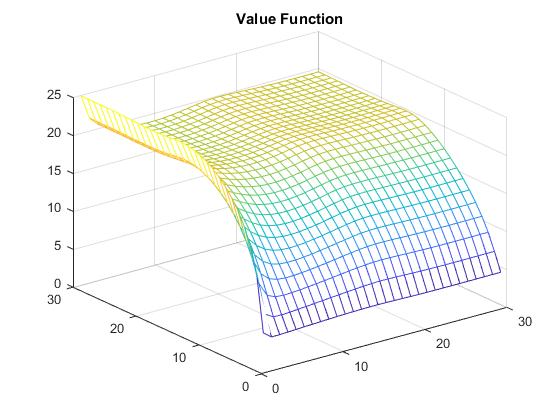
\includegraphics[width=0.75\textwidth]{value.png}
\end{center}
\end{figure}

\begin{figure}[h]
\begin{center}
\caption{Policy function}
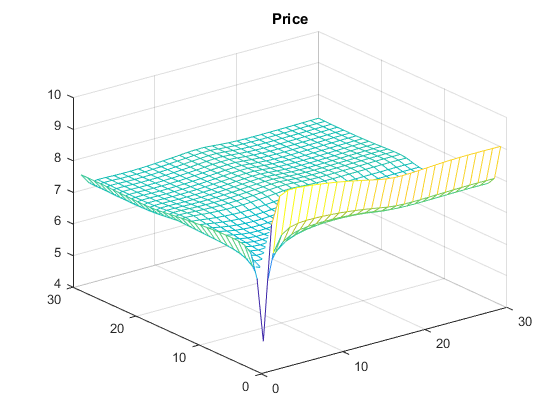
\includegraphics[width=0.75\textwidth]{price.png}
\end{center}
\end{figure}


\newpage
%%%%%%%%%%%%%%%%%%%%%%
\section*{Problem 2}

In main code, I construct $900\times 900$ transition probability matrix which contains $\Pr(\omega_1',\omega_2' |\omega_1,\omega_2)$:

\begin{align*}
&\vect{\rho} = \\
&\bmat{\Pr\prn{{\omega_1^1},{\omega_2^1}| {\omega_1^1},{\omega_2^1} } & \Pr\prn{ {\omega_1^1},{\omega_2^2}| {\omega_1^1},{\omega_2^1} } & \cdots & \Pr\prn{{\omega_1^1},{\omega_2^L}| {\omega_1^1},{\omega_2^1} } &\Pr\prn{{\omega_1^2},{\omega_2^1}| {\omega_1^1},{\omega_2^1} } & \cdots & \Pr\prn{{\omega_1^L},{\omega_2^L}| {\omega_1^1},{\omega_2^1}}\\
\Pr\prn{{\omega_1^1},{\omega_2^1}| {\omega_1^1},{\omega_2^2} } & \Pr\prn{ {\omega_1^1},{\omega_2^2}| {\omega_1^1},{\omega_2^2} } & \cdots & \Pr\prn{{\omega_1^1},{\omega_2^L}| {\omega_1^1},{\omega_2^2} }& \Pr\prn{{\omega_1^2},{\omega_2^1}| {\omega_1^1},{\omega_2^2} }  &\cdots  & \Pr\prn{{\omega_1^L},{\omega_2^L}| {\omega_1^1},{\omega_2^2} }\\
\cdots & \vdots & \vdots & \vdots & \vdots & \vdots\\
\Pr\prn{{\omega_1^1},{\omega_2^1}| {\omega_1^1},{\omega_2^L} } & \Pr\prn{ {\omega_1^1},{\omega_2^2}| {\omega_1^1},{\omega_2^L} } & \cdots & \Pr\prn{{\omega_1^1},{\omega_2^L}| {\omega_1^1},{\omega_2^L} }& \Pr\prn{{\omega_1^2},{\omega_2^1}| {\omega_1^1},{\omega_2^L} }  &\cdots  & \Pr\prn{{\omega_1^L},{\omega_2^L}| {\omega_1^1},{\omega_2^L} }\\
\Pr\prn{{\omega_1^1},{\omega_2^1}| {\omega_2^2},{\omega_2^1} } & \Pr\prn{ {\omega_1^1},{\omega_2^2}| {\omega_2^2},{\omega_2^1} } & \cdots & \Pr\prn{{\omega_1^1},{\omega_2^L}| {\omega_2^2},{\omega_2^1} }& \Pr\prn{{\omega_1^2},{\omega_2^1}| {\omega_2^2},{\omega_2^1} }  &\cdots  & \Pr\prn{{\omega_1^L},{\omega_2^L}| {\omega_2^2},{\omega_2^1} }\\
\cdots & \vdots & \vdots & \vdots & \vdots & \vdots\\
\Pr\prn{{\omega_1^1},{\omega_2^1}| {\omega_2^L},{\omega_2^L} } & \Pr\prn{ {\omega_1^1},{\omega_2^2}|  {\omega_2^L},{\omega_2^L}} & \cdots & \Pr\prn{{\omega_1^1},{\omega_2^L}|  {\omega_2^L},{\omega_2^L}}& \Pr\prn{{\omega_1^2},{\omega_2^1}| {\omega_2^L},{\omega_2^L}} & \cdots  & \Pr\prn{{\omega_1^L},{\omega_2^L}| {\omega_2^L},{\omega_2^L}}\\}
\end{align*}

In order to construct  $\Pr(\omega_1',\omega_2' |\omega_1,\omega_2)$, I use the following relationship
\begin{align*}
 \Pr(\omega_1',\omega_2' |\omega_1,\omega_2)&= \Pr(\omega_1',\omega_2' |\omega_1,\omega_2,q_1,q_2)\Pr(q_1,q_2 |\omega_1,\omega_2)\\
 &=  \Pr(\omega_1' |\omega_1,q_1)\Pr(\omega_2' |\omega_2,q_2)\Pr(q_1,q_2 |\omega_1,\omega_2)
\end{align*}

and 

\begin{align*}
\Pr(q_1,q_2 |\omega_1,\omega_2) = 
\begin{cases}
D_0 \ \ &\text{if} \ \ \ q_1=q_2=0\\
D_1 \ \ &\text{if} \ \ \ q_1=1,\ q_2=0 \\
D_2 \ \ &\text{if} \ \ \ q_1=0,\ q_2=1
\end{cases}
\end{align*}

Since I know $\Pr(\omega_1' |\omega_1,q_1)$, $\Pr(\omega_2' |\omega_2,q_2)$, and $\Pr(q_1,q_2 |\omega_1,\omega_2)$, we can construct $\vect{Trans}$ using the price matrix obtained in problem 1.

Let the state vector be $\vect{s}\in\mathbb{R}^{1\times900}$  where each element corresponds to unique pair of $(\omega_1,\omega_2)$. For example, the first element is $(\omega_1^1,\omega_2^1)$, the second element is  $(\omega_1^1,\omega_2^L)$, and the last element is  $(\omega_1^L,\omega_2^L)$. Since the initial state is (1,1), let $\vect{s}^1 = [1,0,\cdots,0]$. The probability distribution in period 2 is

\begin{align*}
\vect{s}^2 = \vect{\rho}\vect{s}^1
\end{align*}

We can repeat this to get the probability distribution over state in period $t$ as

\begin{align*}
\vect{s}^t =\vect{\rho} \vect{s}^{t-1}
\end{align*}

Following images demonstrate the probability distribution after 10, 20, and 30 periods.


\begin{figure}[h]
\begin{center}
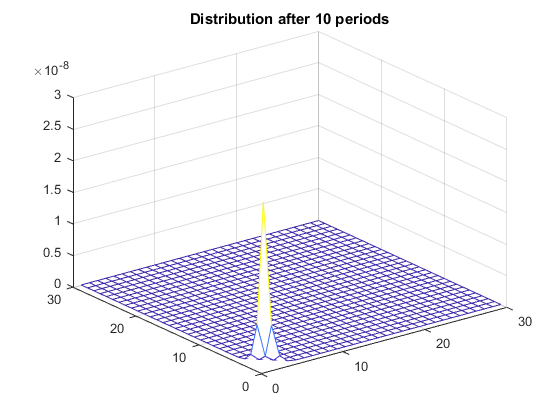
\includegraphics[width=0.75\textwidth]{10period.png}
\end{center}
\end{figure}

\begin{figure}[h]
\begin{center}
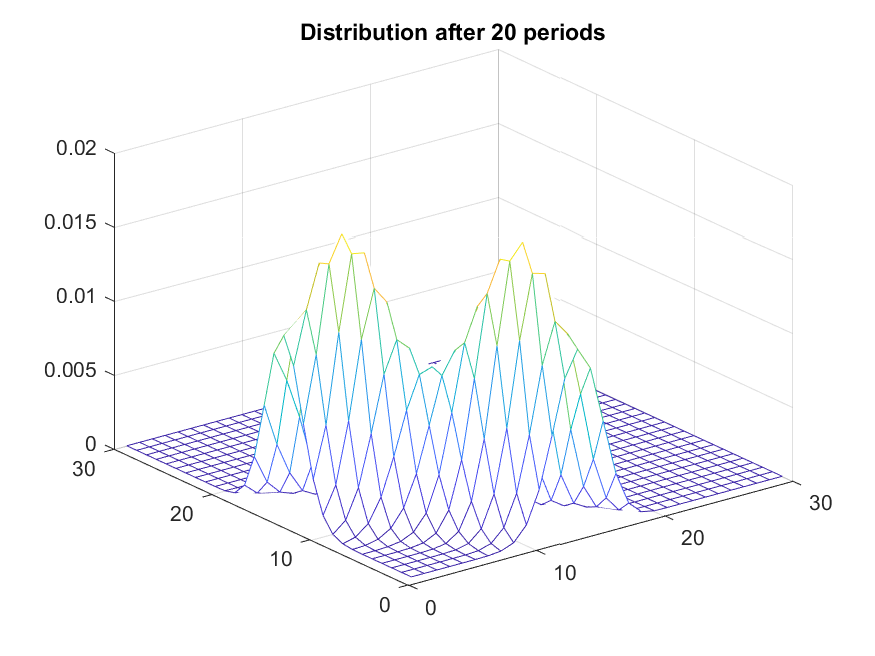
\includegraphics[width=0.75\textwidth]{20period.png}
\end{center}
\end{figure}


\begin{figure}[h]
\begin{center}
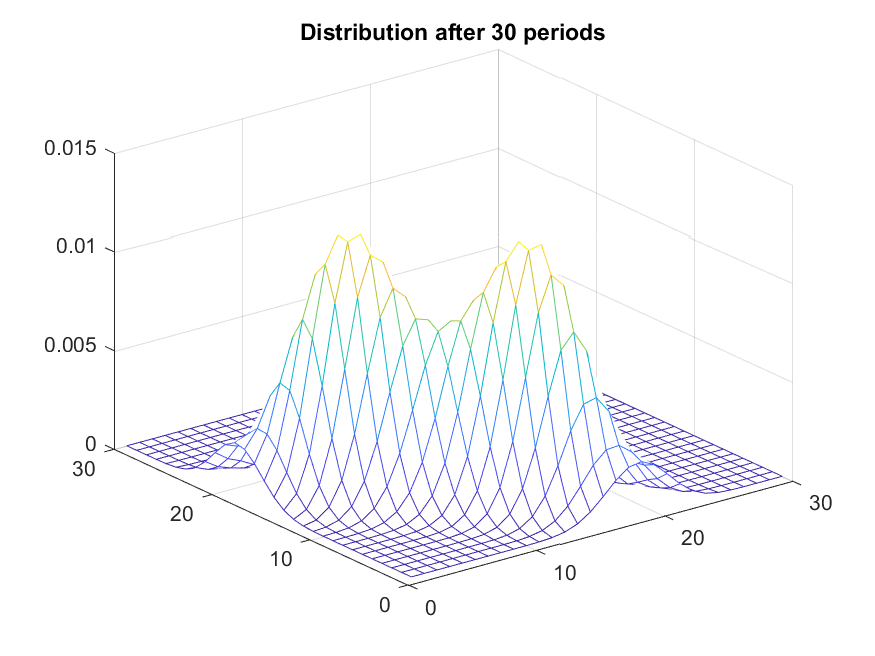
\includegraphics[width=0.75\textwidth]{30period.png}
\end{center}
\end{figure}

\newpage
%%%%%%%%%%%%%%%%%%%%%%
\section*{Problem 3}

Stationary distribution is obtained by iterating

\begin{align*}
\vect{s}^t = \vect{\rho}\vect{s}^{t-1}
\end{align*}

 for $t=2,3,....$ until $\vect{s}^t = \vect{s}^{t+1}$


\begin{figure}[h]
\begin{center}
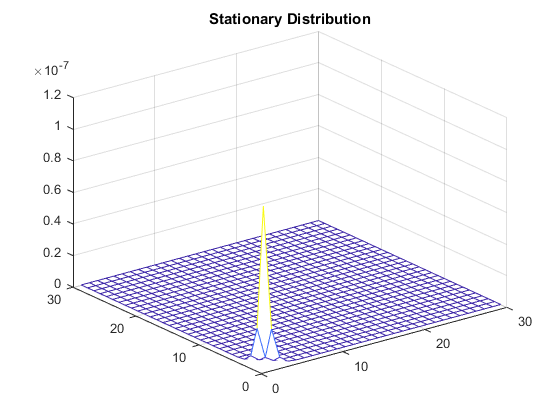
\includegraphics[width=0.75\textwidth]{stationary.png}
\end{center}
\end{figure}

\newpage
%%%%%%%%%%%%%%%%%%%%%%
\section*{Matlab Main Code}
\lstinputlisting{main.m}


\end{document}  



  